\section{Results}
\subsection{Reference-force fidelity of capped fragments}
The calibration evaluates six settings on seven sites from four C16
parents: three perturbation sites and four normal-control sites.
The resulting 42 specifications require 22 distinct
fragment calculations because some settings produce identical fragments.
Figure~\ref{fig:fidelity} and Table~\ref{tab:calibration} show the results.
The smallest graph setting, two bond hops, has a pooled component RMSE
of 0.0278~\forceunit\ but a maximum vector error of
0.2125~\forceunit. It therefore fails the maximum-error criterion despite
passing the pooled-RMSE criterion. All five larger settings pass both.

The radial setting with a 1.5~\AA\ core and 3~\AA\ buffer has
calibration RMSE 0.0118~\forceunit, maximum error 0.0747~\forceunit,
and mean fragment size 28.6 atoms. It ties the three-hop graph setting
in measured mean cost because the retained fragment structures coincide
in this calibration, although their core definitions differ. The fixed
tie rule selects the radial setting. This choice is a cost-constrained
selection among settings that pass, rather than a claim that the chosen
setting minimizes force error.

\begin{figure}[tb]
  \centering
  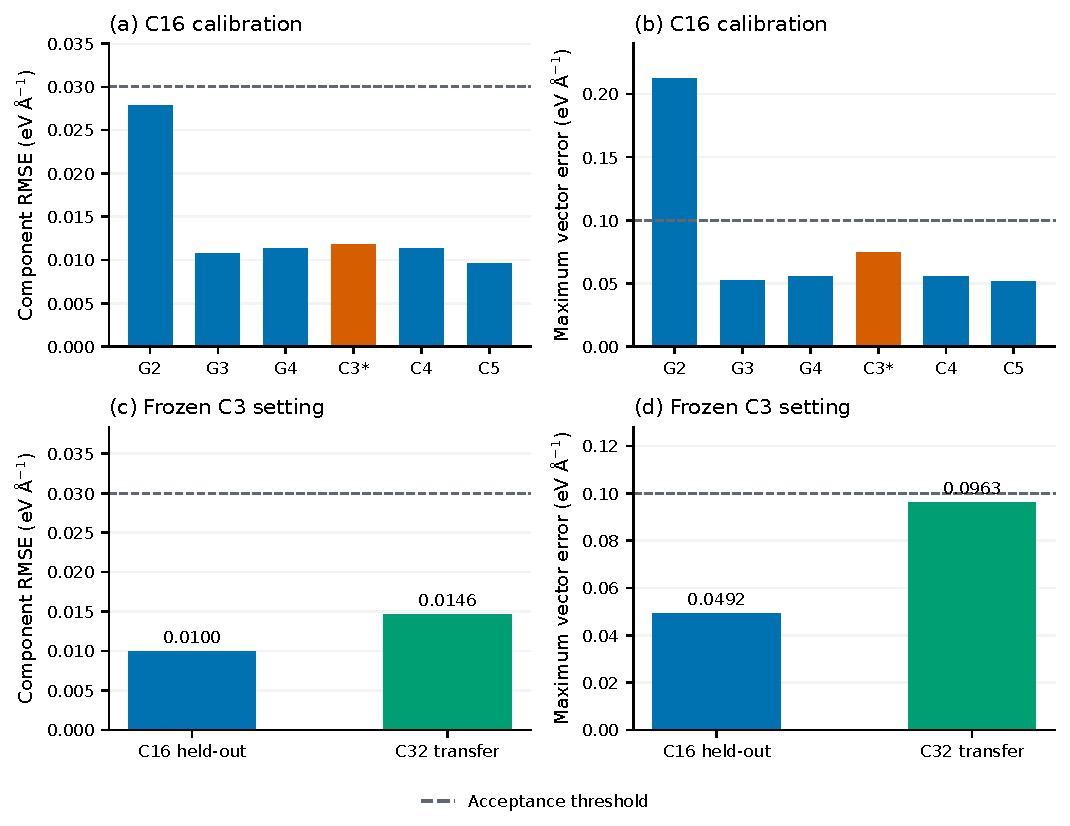
\includegraphics[width=\linewidth]{figures/fig03_fragment_fidelity.pdf}
  \caption{Fragment-fidelity calibration and transfer. G2--G4 denote
  graph neighborhoods of two to four bond hops; C3--C5 denote radial
  neighborhoods with a 1.5~\AA\ core and 3--5~\AA\ buffers. C3*, in
  orange, is selected by the recorded cost-and-tie rule. Upper panels
  show calibration; lower panels apply that setting to held-out C16
  and to two C32 parents. Dashed lines show the component-RMSE and
  maximum-vector-error acceptance thresholds. Bars are pooled
  deterministic evaluations of the available core atoms, not estimates
  with independent statistical error bars.}
  \label{fig:fidelity}
\end{figure}

\begin{table}[tb]
  \centering
  \small
  \caption{C16 calibration. Force errors are in \forceunit.
  Atom counts and allocated core-seconds are means over fragment
  specifications, including repeated structures.}
  \label{tab:calibration}
  \begin{tabular}{lrrrr}
\toprule
Setting & RMSE & Max.\ error & Mean atoms & Core-s/fragment \\
\midrule
Graph, 2 hops & 0.0278 & 0.2125 & 23.7 & 508 \\
Graph, 3 hops & 0.0108 & 0.0521 & 28.6 & 692 \\
Graph, 4 hops & 0.0113 & 0.0552 & 32.9 & 904 \\
Radial, 3 \AA\ buffer (selected) & 0.0118 & 0.0747 & 28.6 & 692 \\
Radial, 4 \AA\ buffer & 0.0113 & 0.0552 & 33.6 & 879 \\
Radial, 5 \AA\ buffer & 0.0095 & 0.0515 & 37.9 & 1095 \\
\bottomrule
\end{tabular}

\end{table}

Applied unchanged to seven sites from four held-out C16 parents, the
selected setting gives RMSE 0.0100~\forceunit\ and maximum error
0.0492~\forceunit. Four fragments from the two C32 parents give
0.0146 and 0.0963~\forceunit, respectively. Both pass, but the C32
maximum is close to the 0.10~\forceunit\ limit. Mean fragment size
increases from 28.6 to 33.3 atoms while the parent size increases from
50 to 98 atoms. This is a small transfer check across two chain lengths,
not a demonstration of asymptotic size independence.

Figure~\ref{fig:cost}(a) separates per-atom core errors by element and
distance to the cut. Carbon and hydrogen occupy different error ranges;
pooling them into a single component RMSE can hide the larger carbon
errors. The maximum-vector criterion supplies a complementary check.
The scatter does not by itself isolate a causal boundary effect from
element, conformation, or perturbation-site differences.

\begin{figure}[tb]
  \centering
  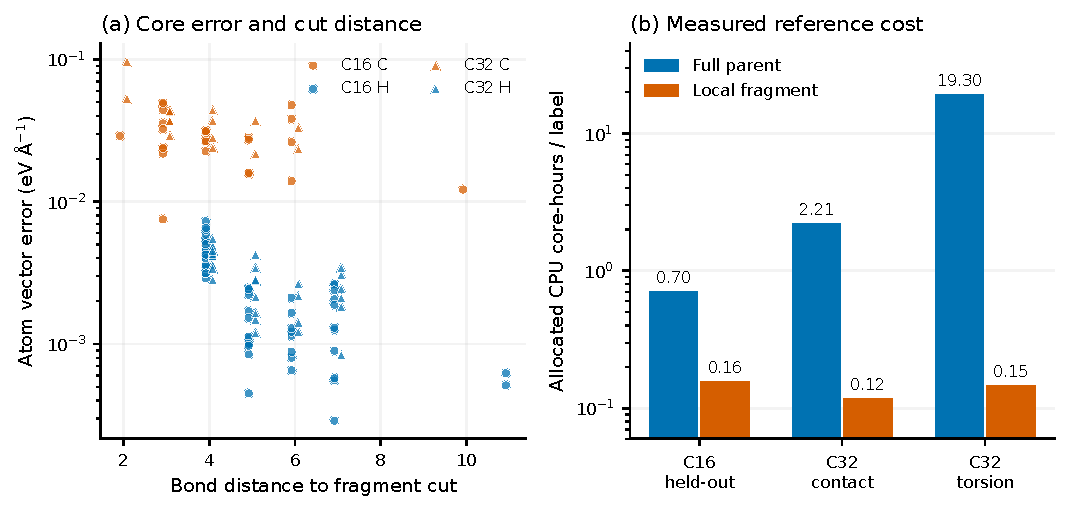
\includegraphics[width=\linewidth]{figures/fig04_boundary_and_cost.pdf}
  \caption{Core-force errors and reference cost for the selected
  fragment setting. (a) Each point is a retained core atom in one
  evaluated fragment; repeated atoms across sites remain separate.
  Horizontal offsets separate C16 circles from C32 triangles.
  Colors distinguish carbon and hydrogen. (b) Allocated cost includes
  all reference attempts. C16 bars are means over the seven held-out
  site specifications, so parents can enter repeatedly. Each C32 full
  bar is one parent calculation, and each local bar averages its two
  fragment calculations. Different box sizes and full-parent SCF
  retries contribute to the large C32 cost differences.}
  \label{fig:cost}
\end{figure}

The held-out C16 mean cost is 0.156~\coreh\ per fragment versus
0.704~\coreh\ for its corresponding full parent, using the
site-weighted means in Fig.~\ref{fig:cost}(b). On C32, the contact
parent costs 2.21~\coreh\ and its fragments average 0.117~\coreh;
the torsional parent costs 19.30~\coreh\ and its fragments average
0.146~\coreh. Both C32 parent jobs require an SCF retry, whereas
the four fragments do not. The parent box edges also differ, at
32.4 and 46.2~\AA. These measurements demonstrate a lower reference
cost for these particular fragments. They do not establish a general
speedup factor or a scaling law for CP2K.

\subsection{Exploratory acquisition comparison}
Figure~\ref{fig:acquisition} retains the individual trajectories of
both repetitions for all five arms. At four acquired labels,
PHAL local and PHAL full have mean held-out force RMSEs of
0.479 and 0.502~\forceunit\ (Table~\ref{tab:acquisition}). Their
mean attributed reference costs are 1948 and 10037 allocated
core-seconds, giving a local/full ratio of 0.194.
The four acquisitions coincide at the parent-and-site level in
the first repetition. They do not fully coincide in the second:
local selection acquires two sites of an ordinary parent, while
full-parent deduplication substitutes a bent parent for the second
ordinary-parent site. Thus the comparison is neither a strictly
paired test of fragment substitution nor a statistical equivalence test.

\begin{figure}[tb]
  \centering
  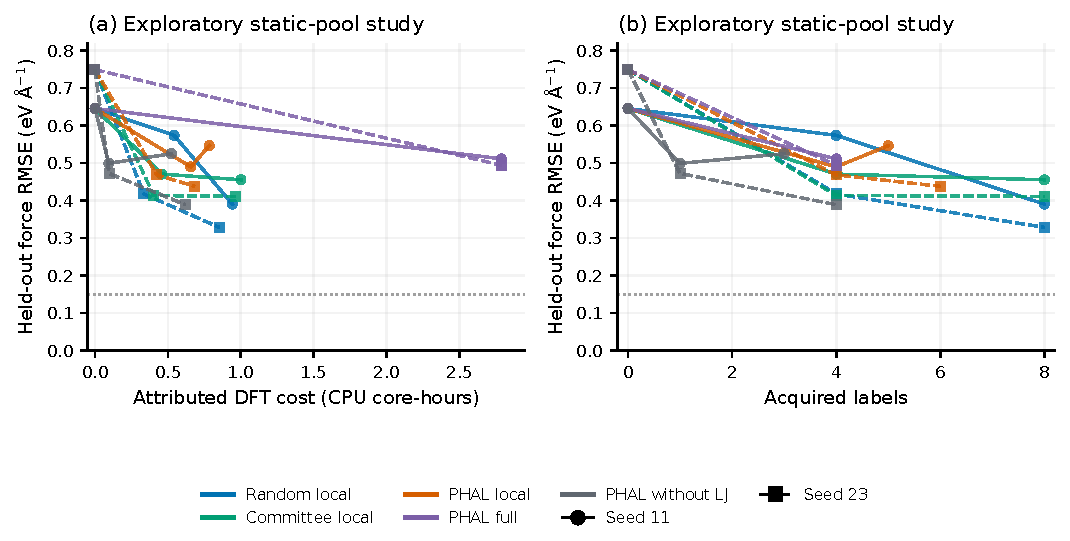
\includegraphics[width=\linewidth]{figures/fig05_acquisition.pdf}
  \caption{Completed exploratory static-pool acquisition study (v2c).
  Each marker is an evaluated model after an acquisition round;
  lines connect observations only and are not additional measurements.
  Solid circles and dashed squares identify the two seeds.
  The horizontal axes show attributed DFT cost and acquired label count.
  Costs charge cached labels at their historical measured reference cost;
  they exclude training, monitoring, and the shared initial dataset.
  The dotted line is the 0.15~\forceunit\ target, which no arm reaches.
  Parent deduplication stops the full-system arm after four labels.
  The final-evaluation set was inspected in earlier exploratory versions.}
  \label{fig:acquisition}
\end{figure}

\begin{table}[tb]
  \centering
  \small
  \caption{Directly observed four-label comparison. Force RMSEs are
  in \forceunit; costs are allocated core-seconds attributed to newly
  acquired labels. Arithmetic means summarize two repetitions without
  implying confidence intervals or equivalence.}
  \label{tab:acquisition}
  \begin{tabular}{lrrrr}
\toprule
Arm & \multicolumn{2}{c}{RMSE at four labels} & Mean RMSE & Mean core-s \\
& Seed 11 & Seed 23 & & \\
\midrule
Random local & 0.5736 & 0.4174 & 0.4955 & 1580 \\
Committee local & 0.4704 & 0.4132 & 0.4418 & 1554 \\
PHAL local & 0.4896 & 0.4683 & 0.4790 & 1948 \\
PHAL full & 0.5110 & 0.4937 & 0.5023 & 10037 \\
\bottomrule
\end{tabular}

\end{table}

Neither PHAL arm consistently outperforms the simpler acquisition
rules. At four labels the committee-ranked arm has mean RMSE
0.442~\forceunit, below the PHAL-local mean. After two rounds,
random acquisition reaches 0.390 and 0.328~\forceunit\ with eight
labels, whereas PHAL local reaches 0.546 and 0.438~\forceunit\ with
five and six labels. These final points have different acquisition
counts and costs. The first PHAL-local repetition worsens after its
second round. No arm reaches either recorded target, 0.15 or
0.10~\forceunit.

Removing the LJ residual reduces triggered structure--round evaluations
from eight of eight in each PHAL-local repetition to three of eight
and four of eight. These eight evaluations comprise four configurations
scored in each of two rounds. Its final errors, 0.525 and
0.389~\forceunit, do not
demonstrate an accuracy benefit from retaining that residual.
The feature affects acquisition behavior, but its incremental
predictive value is unresolved at this sample size.

\subsection{Real closed-loop execution and short-trajectory behavior}
The online pilot executes two GMD segments, collects ten events,
adds three CP2K fragment labels, and promotes two candidate models.
The first update occurs after 1~ps and supplies the second MD
segment. The second update occurs at 2~ps, after the online
trajectory has ended; it is evaluated in the separate frozen-model
trajectories. The fragments contain 44, 26, and 29 atoms and cost
1.054~\coreh\ in total. Validation force RMSE changes from
0.506 to 0.460 to 0.398~\forceunit, a 21.4\% reduction from the
initial value (Fig.~\ref{fig:closed}).

\begin{figure}[tb]
  \centering
  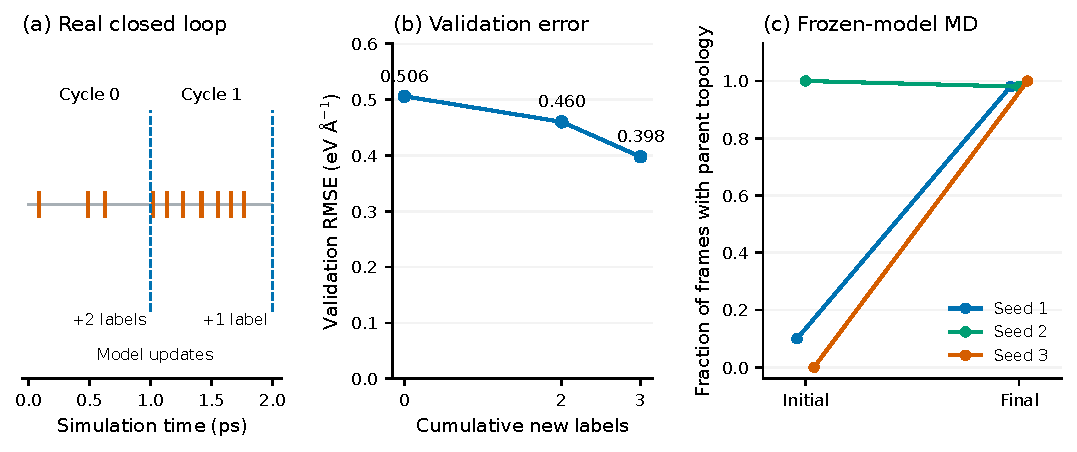
\includegraphics[width=\linewidth]{figures/fig06_closed_loop.pdf}
  \caption{Real-program closed-loop pilot. (a) Orange ticks mark
  recorded events; blue dashed lines mark cycle boundaries at which
  two and then one local labels are incorporated. (b) Validation
  force RMSE after the initial model and the two promotions.
  (c) Fraction of sampled frames retaining the original bond topology
  for each of three velocity seeds under the frozen initial and final
  models. Each point summarizes 151 correlated frames from one short
  trajectory; the points are not independent-frame survival estimates.
  The final model is produced at the end of panel (a) and is tested
  separately in panel (c).}
  \label{fig:closed}
\end{figure}

In the frozen-model evaluation, the initial model retains the
parent topology in 15, 151, and 0 of 151 analyzed frames for the
three seeds. The final model retains it in 148, 148, and 151 frames.
The pooled descriptive fractions are therefore 36.6\% and 98.7\%.
This is an improvement in short-trajectory topology retention, with
brief departures still present under the final model. Frame
autocorrelation and only three trajectories preclude treating the
453 frames as independent replicates. Because the initial model
already fails on an ordinary starting structure, the example does
not establish repair of a qualified model outside its training domain.

Triggering is frequent even on the ordinary initial trajectory.
All ten recorded events include force, committee, and LJ reasons.
In the second cycle, the diversity filter rejects six of seven
candidates and the remaining candidate is labeled. The label budget
and duplicate filter therefore have a substantial role in controlling
reference cost. These records demonstrate working event-to-label
selection, but not a low false-alarm rate.

\subsection{Recovery and rollback}
Separate local fault-injection runs exercise the persistent controller
against real external programs. After termination of the controller
while CP2K remains alive, restart adopts the existing task, collects
its label once, trains and promotes a candidate, and resumes MD.
No extra task directory or duplicate reference attempt is created
in this case. A subsequent deliberately strict validation-gate audit
rejects the promoted model and restores the original accepted model
before MD resumes.
A CP2K cancellation probe passes its eight recorded checks, including
termination and absence of automatic resubmission. These are concrete
integration checks on the local five-thread backend, not evidence
for every scheduler or multi-node failure scenario.
